% Options for packages loaded elsewhere
\PassOptionsToPackage{unicode}{hyperref}
\PassOptionsToPackage{hyphens}{url}
\PassOptionsToPackage{dvipsnames,svgnames,x11names}{xcolor}
%
\documentclass[
  number]{elsarticle}

\usepackage{amsmath,amssymb}
\usepackage{iftex}
\ifPDFTeX
  \usepackage[T1]{fontenc}
  \usepackage[utf8]{inputenc}
  \usepackage{textcomp} % provide euro and other symbols
\else % if luatex or xetex
  \usepackage{unicode-math}
  \defaultfontfeatures{Scale=MatchLowercase}
  \defaultfontfeatures[\rmfamily]{Ligatures=TeX,Scale=1}
\fi
\usepackage{lmodern}
\ifPDFTeX\else  
    % xetex/luatex font selection
\fi
% Use upquote if available, for straight quotes in verbatim environments
\IfFileExists{upquote.sty}{\usepackage{upquote}}{}
\IfFileExists{microtype.sty}{% use microtype if available
  \usepackage[]{microtype}
  \UseMicrotypeSet[protrusion]{basicmath} % disable protrusion for tt fonts
}{}
\makeatletter
\@ifundefined{KOMAClassName}{% if non-KOMA class
  \IfFileExists{parskip.sty}{%
    \usepackage{parskip}
  }{% else
    \setlength{\parindent}{0pt}
    \setlength{\parskip}{6pt plus 2pt minus 1pt}}
}{% if KOMA class
  \KOMAoptions{parskip=half}}
\makeatother
\usepackage{xcolor}
\setlength{\emergencystretch}{3em} % prevent overfull lines
\setcounter{secnumdepth}{5}
% Make \paragraph and \subparagraph free-standing
\ifx\paragraph\undefined\else
  \let\oldparagraph\paragraph
  \renewcommand{\paragraph}[1]{\oldparagraph{#1}\mbox{}}
\fi
\ifx\subparagraph\undefined\else
  \let\oldsubparagraph\subparagraph
  \renewcommand{\subparagraph}[1]{\oldsubparagraph{#1}\mbox{}}
\fi


\providecommand{\tightlist}{%
  \setlength{\itemsep}{0pt}\setlength{\parskip}{0pt}}\usepackage{longtable,booktabs,array}
\usepackage{calc} % for calculating minipage widths
% Correct order of tables after \paragraph or \subparagraph
\usepackage{etoolbox}
\makeatletter
\patchcmd\longtable{\par}{\if@noskipsec\mbox{}\fi\par}{}{}
\makeatother
% Allow footnotes in longtable head/foot
\IfFileExists{footnotehyper.sty}{\usepackage{footnotehyper}}{\usepackage{footnote}}
\makesavenoteenv{longtable}
\usepackage{graphicx}
\makeatletter
\def\maxwidth{\ifdim\Gin@nat@width>\linewidth\linewidth\else\Gin@nat@width\fi}
\def\maxheight{\ifdim\Gin@nat@height>\textheight\textheight\else\Gin@nat@height\fi}
\makeatother
% Scale images if necessary, so that they will not overflow the page
% margins by default, and it is still possible to overwrite the defaults
% using explicit options in \includegraphics[width, height, ...]{}
\setkeys{Gin}{width=\maxwidth,height=\maxheight,keepaspectratio}
% Set default figure placement to htbp
\makeatletter
\def\fps@figure{htbp}
\makeatother

\usepackage{booktabs}
\usepackage{longtable}
\usepackage{array}
\usepackage{multirow}
\usepackage{wrapfig}
\usepackage{float}
\usepackage{colortbl}
\usepackage{pdflscape}
\usepackage{tabu}
\usepackage{threeparttable}
\usepackage{threeparttablex}
\usepackage[normalem]{ulem}
\usepackage{makecell}
\usepackage{xcolor}
\usepackage{siunitx}

  \newcolumntype{d}{S[
    input-open-uncertainty=,
    input-close-uncertainty=,
    parse-numbers = false,
    table-align-text-pre=false,
    table-align-text-post=false
  ]}
  
\makeatletter
\@ifpackageloaded{caption}{}{\usepackage{caption}}
\AtBeginDocument{%
\ifdefined\contentsname
  \renewcommand*\contentsname{Table of contents}
\else
  \newcommand\contentsname{Table of contents}
\fi
\ifdefined\listfigurename
  \renewcommand*\listfigurename{List of Figures}
\else
  \newcommand\listfigurename{List of Figures}
\fi
\ifdefined\listtablename
  \renewcommand*\listtablename{List of Tables}
\else
  \newcommand\listtablename{List of Tables}
\fi
\ifdefined\figurename
  \renewcommand*\figurename{Figure}
\else
  \newcommand\figurename{Figure}
\fi
\ifdefined\tablename
  \renewcommand*\tablename{Table}
\else
  \newcommand\tablename{Table}
\fi
}
\@ifpackageloaded{float}{}{\usepackage{float}}
\floatstyle{ruled}
\@ifundefined{c@chapter}{\newfloat{codelisting}{h}{lop}}{\newfloat{codelisting}{h}{lop}[chapter]}
\floatname{codelisting}{Listing}
\newcommand*\listoflistings{\listof{codelisting}{List of Listings}}
\makeatother
\makeatletter
\makeatother
\makeatletter
\@ifpackageloaded{caption}{}{\usepackage{caption}}
\@ifpackageloaded{subcaption}{}{\usepackage{subcaption}}
\makeatother
\ifLuaTeX
  \usepackage{selnolig}  % disable illegal ligatures
\fi
\usepackage[]{natbib}
\usepackage{bookmark}

\IfFileExists{xurl.sty}{\usepackage{xurl}}{} % add URL line breaks if available
\urlstyle{same} % disable monospaced font for URLs
\hypersetup{
  pdftitle={(No) Privacy Please!: What Determines Chinese Attitudes Toward Online Government Monitoring},
  pdfkeywords={Digital Privacy, Covid-19, Authoriatrian
Regimes, Government Trust, China},
  colorlinks=true,
  linkcolor={blue},
  filecolor={Maroon},
  citecolor={Blue},
  urlcolor={Blue},
  pdfcreator={LaTeX via pandoc}}

\setlength{\parindent}{6pt}
\begin{document}

\begin{frontmatter}
\title{(No) Privacy Please!: What Determines Chinese Attitudes Toward
Online Government Monitoring}


\cortext[cor1]{Corresponding author}
        
\begin{abstract}
This study investigates the determinants of public opinion toward
government monitoring in China. The existing literature on the
acceptance of government monitoring raises several open questions,
including the extent to which demographic variables influence the
relationship, how government trust relates to the acceptance of
government monitoring, and whether the acceptance of public versus
private monitoring shares the same determinants. Using a two-wave survey
conducted before and after the Covid-19 lockdowns in China, the study
finds that: 1) demographic factors do not seem to be related to the
acceptance of government monitoring; 2) government trust does predict
attitudes, although the Covid-19 experience has significantly modified
this relationship; and 3) the acceptance of private monitoring appears
to have different determinants. The study concludes by considering some
implications of these findings.
\end{abstract}





\begin{keyword}
    Digital Privacy \sep Covid-19 \sep Authoriatrian
Regimes \sep Government Trust \sep 
    China
\end{keyword}
\end{frontmatter}
    
\section{Introduction}\label{sec-introduction}

The dramatic events of the Covid-19 era have brought to the forefront
citizens' relationships with government tracking technologies. Users
were often required to install government apps that monitored their
location, the stores they entered, and even whether they purchased cold
medicines \citep{mcmorrow2022}. Nowhere was this tracking more invasive
than in China, where the government mobilized technological tools to
deeply peer into the daily lives of its citizens. The impact of these
events on users' attitudes toward technological monitoring has not yet
been fully described. Utilizing a unique dataset, this study resolves
several open questions in the literature regarding how citizens view
government monitoring.

Citizens' attitudes toward government intrusions into their online
privacy is an understudied area, with numerous unanswered questions in
the literature \citep{gómez-barroso2018}, particularly regarding how
citizens view this topic in authoritarian and non-Western contexts. One
unresolved question is the extent to which demographic or privacy
knowledge variables predict attitudes. Literature on general privacy
offers several suggestions as to which variables may shape attitudes,
but little research has been undertaken to determine if these findings
apply to attitudes toward government monitoring. To the extent that
there is consensus in the literature, it agrees that government trust
should be strongly related to attitudes toward government tracking.
However, this literature has not reached a consensus on how an event
like the Covid-19 lockdowns might alter this relationship, nor has it
provided direct causal tests of the relationship. Furthermore, it is not
clear whether the variables that predict attitudes toward government
tracking should also predict attitudes toward private tracking.

To address these gaps in the literature, this study utilizes two waves
of a survey conducted before and after the 2022 Covid-19 lockdowns in
China to develop models of respondents' attitudes. The first model
examines a set of demographic and technology knowledge variables as
predictors for acceptance of government tracking and finds that the
models are poor fits, with few variables achieving statistical or
substantive significance. The second set of models adds government trust
as a predictor variable and finds, as expected, that government trust is
an important predictor of attitudes. A mediation model is then developed
that separates the direct effect of Covid-19 on attitudes toward
government tracking from the indirect effect of Covid-19 on government
trust, which subsequently influences attitudes toward government
monitoring. This mediation model finds that the overall effect of
Covid-19 is positive but complex, with the direct and indirect effects
operating in opposing directions. Finally, the paper examines a model to
test whether any of the predictor variables for public tracking can
predict attitudes toward private tracking; the model's results suggest
that they cannot.

Taken together, these results indicate that government trust matters but
what may be equally important is the public perception of the rationale
for government tracking. The conclusion discusses these results in the
context of the existing literature and highlights some important
implications and areas for future research.

\section{Literature review}\label{sec-litreview}

\subsection{Background}\label{background}

What predicts respondents' attitudes toward government tracking of their
online activity has generated significant scholarly interest in the last
ten years, yet the findings have not reached any firm conclusions on a
number of important questions \citep{reddick2015}. Compounding this
issue, to date, most research on the topic has been conducted primarily
with U.S. or Western respondents, with comparatively fewer studies
reporting on developing or non-democratic countries. This research
agenda has gained new urgency during the Covid-19 pandemic, as
governments around the world have engaged in highly intrusive monitoring
and data collection activities.

From the pre-Covid privacy literature, two important findings are
prominent. The first is that demographic variables are significant
predictors of attitudes toward generalized online privacy. In a notable
early study of early Internet users, Sheehan found that education and
age are two significant determinants of online privacy attitudes
\citep{sheehan2002}. Others have replicated this result and found that
characteristics such as gender, social setting, and income also play a
role in forming privacy expectations
\citep{anwar2017, büchi2021, lee2019}. The second finding is that
respondents' personal experience with privacy and technology is also an
important factor in predicting privacy attitudes. Baskaran and Mathew
report that users with significant knowledge of and interest in privacy
have a greater fear of losing their privacy, and this fear motivates
them to change their online behavior \citep{baskaran2024}. Dupree et
al.~suggest that various possible online user typologies exist, with
user experience being a significant variable that matters that can
potentially shift respondents to an extreme view in either direction
\citep{dupree2016}. Kokolakis, as part of a meta-analysis of privacy,
notes that young people may be more aware of their online privacy
context and therefore more active in policing their privacy boundaries
\citep{kokolakis2017}, a finding that Blank et al.~have replicated
\citep{blank}. These findings suggest that personal characteristics and
background are important determinants of privacy attitudes, though how
these findings relate to government monitoring specifically remains
unclear.

The second key finding is that trust in the state is a significant
correlate of whether respondents feel anxious about government
monitoring of their online behavior. Davis and Silver discovered that
Americans with lower levels of trust in the government were less willing
to accept government surveillance programs after the 9/11 terrorist
attacks \citep{davis2004}. Pavone and Esposti determined that users
either trusted the government and therefore did not find proposed
monitoring concerning, or they did not trust the government and thus
perceived any monitoring as threatening \citep{pavone2012}. Trüdinger
and Steckermeier found that acceptance of government surveillance in
Germany depends on how much respondents trust the state
\citep{trüdinger2017}. However, this literature has so far been unable
to causally link trust and acceptance of monitoring. It is possible that
acceptance of government monitoring is downstream of government trust,
but it could also be that government trust and monitoring are both
influenced by personality or demographic attributes. It is also unclear
from these studies how rapidly or under what types of events might
change government trust and then whether that change in trust would
subsequently alter attitudes toward acceptance of government tracking.

The literature on government monitoring of citizens increased
dramatically following the onset of the Covid-19 pandemic, though most
findings echo those of Pavone and Esposti and other earlier scholars.
Because the Covid-19 pandemic introduced a wide array of new tracking
technologies, scholars have focused directly on users' and respondents'
feelings regarding government monitoring (for a sampling of the
extensive literature, see
\citep{abramova2022, garrett2021, ioannou2021, ong, wnuk2020}). To
highlight one example of Covid-era research, Ioannou and Tussyadiah
linked state trust, surveillance acceptance, and perceived necessity in
explaining the variation in willingness to use contact tracing apps in
the U.S. Generally, this research finds that Covid-19 is an important
factor in shaping views on tracking. However, most of this research
tests acceptance of specific monitoring technologies (such as vaccine
passports) or examines attitudes only in close temporal proximity to the
technology's usage and therefore offers limited information about the
durability of these attitudes.

Additionally, how these findings translate to the Chinese context is not
obvious. While recent research has begun to develop a picture of Chinese
attitudes towards government monitoring, some important questions remain
unanswered. Several studies have found that Chinese respondents are
generally more willing to use or accept government surveillance
technologies across various technology types
\citep{habich-sobiegalla2023, kostka2021, kostka2024}. Liu and Kostka,
in separate studies, both establish that trust in the state correlates
with increased acceptance of the social credit system (Liu) and
surveillance broadly (Kostka) \citep{kostka2023, liu2022}. However, to
date, there have been no major studies that have conducted a
before-and-after analysis of attitude change as a result of China's
Covid-19 experiences.

Finally, a line of research investigates whether differences in
attitudes exist if the surveillance is conducted by the government
versus a private entity. Steinfeld finds differences in attitudes
between the two, with the justification for surveillance being a key
factor for government monitoring acceptance (accepting the War on Terror
as essential) and compensatory benefits being the strongest predictor of
private monitoring acceptance \citep{steinfeld2017}. Nam indicates that
it is primarily demographic features that predict generalized privacy
concerns, while government privacy concerns are chiefly predicted by
trust in the government \citep{nam2019}. These studies both focus on
Americans and therefore it is unclear how generalizable their results
are. Research in China by Steinhardt et al.~finds that users in China
tend to trust the government with their data more than they do private
corporations, but does not explore the specific determinants of this
variation in trust \citep{steinhardt2022}.

\subsection{Contribution}\label{contribution}

This work aims to make three contributions to the literature on
government surveillance. First, it seeks to clarify which demographic
and attitudinal factors are significant in predicting privacy concerns.
Previous findings have supported the idea that certain respondent
attributes predict acceptance of government surveillance; if these
findings do not find support here, it may suggest that demographics are
a poor fit in explaining respondent attitudes towards government
tracking not just in China.

Second, this study aims to establish to what degree and in what ways
government trust and government privacy attitudes are linked. So far,
there have been very few studies of privacy attitudes that are not
purely cross-sectional. The survey used in this paper was conducted in
two waves, one before the strict Covid-19 controls were implemented in
China, and another wave just after the controls were relaxed, which
helps add additional leverage to explore how events and context may also
matter for shifting attitudes. In particular, during this period, as You
et al.~have found, the Chinese response to the pandemic engendered
significant criticism and resulted in a decline in trust in the
government \citep{you2024}. This study can help determine if government
trust is an important predictor of attitudes, and, if it is, whether a
decline in trust along with event-specific effects mechanically lead to
a lower level of acceptance of government monitoring.

Finally, the study aims to determine whether the factors influencing
acceptance of tracking differ depending on whether the tracking is
conducted by private entities or government organizations. If different
determinants exist, it would imply that users are cognizant of the
political context of government monitoring and that this awareness
shapes their attitudes. This distinction is important given that much of
the existing research on the formation of privacy attitudes focuses on
private monitoring \citep{gómez-barroso2018}.

\subsection{Hypotheses}\label{hypotheses}

The existing literature and the specific features of this survey
generates a set of testable hypotheses, \(H_1\) through \(H_6\).

\(H_1\): Demographic variables such as age, education, and income
predict acceptance of government monitoring

A finding here that certain demographic factors are predictors of
attitudes toward government monitoring can help clarify whether the
demographic linkages found in research on generalized privacy attitudes
or attitudes toward private monitoring are similar for attitudes toward
government monitoring.

\(H_{2a}\) Technical know-how and privacy consciousness predicts
acceptance of government monitoring

\(H_{2b}\): Technical know-how and privacy consciousness does not
predict acceptance of government monitoring

Existing literature finds that those with significant experience or
knowledge of information and communication technologies (ICTs) are more
careful with their online privacy. However, it is also the case that the
Chinese online information environment is highly controlled,
particularly with respect to any information critical of the government
\citep{han2018} so such knowledge may have less of an impact on
attitudes. Government propaganda extolling the benevolence of the state
with regards to protecting users \citep{gainous2023} may even counteract
or reverse the fear effect of greater knowledge of privacy. Therefore,
privacy knowledge and technical skill may also be uncorrelated or even
positively correlated with support for government monitoring.

\(H_3\): Trust in government should predict acceptance of government
monitoring

Both existing studies of Chinese users and those outside of China have
all found this relationship to be a relatively robust one. Research on
China has also found that government trust is an important predictor of
many other social and attitudinal variables
\citep{chen2017, qiu2012, zhou2018}.

\(H_4\): The pandemic should alter the acceptance of government
monitoring

This hypothesis could be true in two different ways. The first way is
via a direct effect - the experience of intrusive and long-lasting
surveillance could lower support for government monitoring. Alternately,
it could increase support for government monitoring if the population
viewed the surveillance as socially beneficial. The second way is via an
indirect effect - the experience of the pandemic could decrease
government trust and then this decrease in trust leads to lower support
for government surveillance.

\(H_5\): Factors that drive concern regarding government tracking should
differ from concerns regarding private tracking

Given that previous research has found significant differences in the
level of acceptance of tracking between public and private sources in
China, and, that trust in government is likely not a factor for
accepting private tracking, there should be differences in the factors
that predict these two variables.

\section{Data and summary statistics}\label{sec-datasummary}

The data for this project were collected via a commercial market
research firm in two waves: February 2021 and March 2023. The first
survey had an n of 1,500 and the second had an n of 2,000. Questions on
the two surveys were identical except for a minor change to a question
that referenced a specific date. The timing of the two surveys coincided
with two very different points in China's Covid-19 experience. The first
survey was conducted approximately seven months after the last round of
restrictions had been lifted in the city of Wuhan. At that time, China
was essentially closed to foreign travel but otherwise had few
day-to-day public health restrictions in place. Nationwide, daily Covid
cases hovered around the single digits \citep{wuhanlo2021}. By March
2023, China found itself at a very different stage. The year 2022 saw
the introduction of widespread, intrusive digital monitoring. Many major
cities, such as Shanghai, Xi'an, and Shenzhen, underwent prolonged and
arduous city-wide lockdowns. At the end of 2022, under the pressure of a
spiraling number of cases and widespread protests (known as the White
Paper Revolution), China finally abandoned its zero-Covid policy
\citep{mao2022}. March 2023 is far enough removed from the end of the
zero-Covid policies for any temporary attitudinal effects of the
lockdowns and monitoring to have subsided, yet it is close enough to the
end of the policy that differences in attitudes can plausibly be
attributed to the Covid-19 experience and not subsequent events. Thus,
these two surveys provide excellent data for examining hypotheses
1-6.\footnote{All code and data to replicate these results available at
  the author's GitHub repository.}

The demographics of the 2021 and 2023 surveys are presented in
Table~\ref{tbl-demographics}.

\begin{longtable}[t]{llrr}

\caption{\label{tbl-demographics}Select key demographic variables}

\tabularnewline

\toprule
  &    & Mean & Std. Dev.\\
\midrule
Age &  & 33.2 & 11.6\\
\midrule
 &  & N & Pct.\\
Location & Countryside/village & 477 & 13.6\\
 & Small city & 1059 & 30.2\\
 & Mid-sized city & 840 & 24.0\\
 & Big city & 1131 & 32.2\\
Education & No formal education & 22 & 0.6\\
 & Primary & 134 & 3.8\\
 & Middle school & 384 & 10.9\\
 & High school & 843 & 24.0\\
 & University & 1914 & 54.6\\
 & Advanced studies/Graduate school & 210 & 6.0\\
Gender & Female & 1711 & 48.8\\
 & Male & 1796 & 51.2\\
Marriage status & Single & 1101 & 31.4\\
 & In a relationship & 569 & 16.2\\
 & Married & 1744 & 49.7\\
 & Divorced & 93 & 2.7\\
Communist Party member status & Yes & 483 & 13.8\\
 & No & 3024 & 86.2\\
Communist Youth League status & Yes & 1116 & 31.8\\
 & No & 2391 & 68.2\\
Income & 0-2,999 & 275 & 7.8\\
 & 3,000-5,999 & 822 & 23.4\\
 & 6,000-9,999 & 899 & 25.6\\
 & 10,000-19,999 & 962 & 27.4\\
 & 20,000-49,999 & 385 & 11.0\\
 & 50,000-99,999 & 94 & 2.7\\
 & More than 100,000 & 70 & 2.0\\
Year & 2021 & 1500 & 42.8\\
 & 2023 & 2007 & 57.2\\
\bottomrule

\end{longtable}

As is typical with online surveys in China, the sample respondents tend
to be younger and more educated. Comparing the two waves, there are some
modest demographic differences (notably in education and marital status)
between the two samples. As will be shown in Section
Section~\ref{sec-analysis}, these minor differences do not seem to alter
any of the substantive results. Focusing on the 2023 survey, the typical
respondent is a male from a small city, married, employed in a
white-collar job at a small enterprise, earning approximately 10,000 RMB
a month, and holding an urban residence permit (hukou). To simplify the
analysis that follows, the variables have been recoded: income is
divided into three categories (low, middle, and high) and education into
two categories, those with a college education and those without. The
regressions in the subsequent sections were tested with alternative
specifications of these categorical variables (the code for these
regressions is available on the author's website), and the key results
remained unchanged.

\begin{table}

\caption{\label{tbl-respvarindex}Questions asking about attitudes toward
government monitoring}

\centering{

\centering
\begin{tabular}[t]{l|>{\raggedright\arraybackslash}p{5in}}
\hline
GM1 & There are good reasons for the central government to monitor the activity of users online\\
\hline
\cellcolor{gray!6}{GM2} & \cellcolor{gray!6}{There are good reasons for the local government to monitor the activity of users online}\\
\hline
TRACK1 & How comfortable are you with the central government knowing personal details about your activity online?\\
\hline
\cellcolor{gray!6}{TRACK2} & \cellcolor{gray!6}{How comfortable are you with the local government knowing personal details about your activity online?}\\
\hline
\end{tabular}

}

\end{table}%

The key response variable for the following analysis is an index
variable created by combining the results of the four questions in
Table~\ref{tbl-respvarindex}, rescaled to be between zero and one. It is
true that previous research has found that Chinese respondents place
lower levels of trust in local governments as compared to central
governments \citep{chen2017, zhong2014}, suggesting there may be some
differences in attitudes between central and local monitoring. However,
the correlation between \texttt{GM1} and \texttt{GM2} is 0.84 and the
correlation between \texttt{TRACK1} and \texttt{TRACK2} is 0.87.
Additionally, as shown in the online appendices, each of the major
regression results in Section~\ref{sec-analysis} do not demonstrate
major changes if the same variables are regressed on each of the index
items individually. Indicating their close relationship, the variables
taken together have a Cronbach's \(\alpha\) of 0.81. Intuitively, this
high level of relatedness makes sense as while respondents have some
background attitudes about the difference between central and local
governments, they may not easily be able to identify at which level
government tracking occurs.

Finally, there has been some debate regarding the extent of preference
falsification of political attitudes in online surveys in China
\citep{carter2024, jiang2016, ratigan2020}. If respondents are afraid to
reveal their true attitudes toward the government, it could potentially
bias the results. To test for preference falsification, the survey
instrument also included several list experiment questions, which
allowed respondents' attitudes to be inferred indirectly without
requiring them to directly state their opinions about the government.
List experiments have been utilized in numerous surveys to offer
residents a confidential method of expressing their true attitudes on
topics such as racial perspectives, experiences of sexual assault, and
political views \citep{redlawsk2010, moseson2017}. Although
\citep{glynn2013} suggests that list experiments should not be viewed as
a panacea for the issue of preference falsification, the results of the
list experiments (detailed in the online appendices) correspond closely
with the answers to the component questions that comprise the response
variable index. Additionally, the topic of this survey is less sensitive
than other, more directly political research, and should therefore be
less likely to provoke significant fear of reprisal among respondents.
Overall, the survey data should provide a robust means to differentiate
between the hypotheses presented in Section~\ref{sec-litreview}.

\section{Analysis}\label{sec-analysis}

\subsection{Predicting citizen attitudes about government
monitoring}\label{predicting-citizen-attitudes-about-government-monitoring}

The first set of models considers the question of which demographic
variables predict variation in attitudes toward being tracked by the
government. Overall, the central finding is that the demographic
variables are relatively weak predictors of acceptance of government
monitoring. The key predictor variables included in
Table~\ref{tbl-citizenatt} are the standard suite of demographic
variables, the tech savvy index (\texttt{TSI}), and the knowledge index
(\texttt{KI}). The items used to construct the two indicies variables
are listed in Section~\ref{sec-appendix}. The Cronbach's \(\alpha\) for
each of the two variables are 0.8 and 0.55 respectively, indicating that
the questions are suitable for use in an index. Additionally, this model
interacts education and sex with \texttt{GPI} - as recent research has
suggested that younger generations have different attitudinal patterns
than older generations \citep{harmel2019, steinhardt2020}, and ICT
knowledge may also differ significantly by gender. Added to the index
variables and the interaction terms are a slate of standard control
variables.

\begin{table}

\caption{\label{tbl-citizenatt}Demographic predictors of attitude toward
government privacy}

\centering{

\centering
\begin{tabular}[t]{lcccccc}
\toprule
  & (1) & (2) & (3) & (4) & (5) & (6)\\
\midrule
(Intercept) & \num{0.573}*** & \num{0.548}*** & \num{0.488}*** & \num{0.506}*** & \num{0.504}*** & \num{0.576}***\\
 & (\num{0.019}) & (\num{0.019}) & (\num{0.021}) & (\num{0.023}) & (\num{0.022}) & (\num{0.022})\\
Age & \num{0.001}*** & \num{0.001}** & \num{0.002}*** & \num{0.001}*** & \num{0.002}*** & \num{0.001}***\\
 & (\num{0.000}) & (\num{0.000}) & (\num{0.000}) & (\num{0.000}) & (\num{0.000}) & (\num{0.000})\\
College education & \num{0.010} & \num{0.014}+ & \num{0.006} & \num{-0.026} & \num{0.006} & \num{0.014}+\\
 & (\num{0.008}) & (\num{0.008}) & (\num{0.008}) & (\num{0.017}) & (\num{0.008}) & (\num{0.008})\\
Middle income & \num{0.000} & \num{0.002} & \num{-0.003} & \num{-0.004} & \num{-0.003} & \num{0.001}\\
 & (\num{0.008}) & (\num{0.008}) & (\num{0.008}) & (\num{0.008}) & (\num{0.008}) & (\num{0.008})\\
High income & \num{-0.015} & \num{-0.012} & \num{-0.024} & \num{-0.025} & \num{-0.024} & \num{-0.014}\\
 & (\num{0.017}) & (\num{0.017}) & (\num{0.017}) & (\num{0.017}) & (\num{0.017}) & (\num{0.017})\\
Male & \num{-0.004} & \num{-0.003} & \num{-0.009} & \num{-0.010} & \num{-0.040}* & \num{-0.004}\\
 & (\num{0.007}) & (\num{0.007}) & (\num{0.007}) & (\num{0.007}) & (\num{0.016}) & (\num{0.007})\\
Not a party member & \num{-0.033}** & \num{-0.034}*** & \num{-0.030}** & \num{-0.029}** & \num{-0.030}** & \num{-0.032}**\\
 & (\num{0.010}) & (\num{0.010}) & (\num{0.010}) & (\num{0.010}) & (\num{0.010}) & (\num{0.010})\\
Location: small city & \num{0.000} & \num{0.002} & \num{-0.003} & \num{-0.001} & \num{-0.003} & \num{0.002}\\
 & (\num{0.011}) & (\num{0.011}) & (\num{0.011}) & (\num{0.011}) & (\num{0.011}) & (\num{0.011})\\
Location: mid city & \num{0.007} & \num{0.009} & \num{0.000} & \num{0.001} & \num{0.000} & \num{0.008}\\
 & (\num{0.012}) & (\num{0.012}) & (\num{0.012}) & (\num{0.012}) & (\num{0.012}) & \vphantom{1} (\num{0.012})\\
Location: big city & \num{0.013} & \num{0.014} & \num{0.001} & \num{0.002} & \num{0.001} & \num{0.013}\\
 & (\num{0.012}) & (\num{0.012}) & (\num{0.012}) & (\num{0.012}) & (\num{0.012}) & (\num{0.012})\\
Year 2023 &  & \num{0.037}*** & \num{0.039}*** & \num{0.038}*** & \num{0.038}*** & \num{0.036}***\\
 &  & (\num{0.007}) & (\num{0.007}) & (\num{0.007}) & (\num{0.007}) & (\num{0.007})\\
TSI &  &  & \num{0.118}*** & \num{0.010} & \num{0.017} & \\
 &  &  & (\num{0.017}) & (\num{0.055}) & (\num{0.052}) & \\
TSI x education &  &  &  & \num{0.069}* &  & \\
 &  &  &  & (\num{0.034}) &  & \\
TSI x sex &  &  &  &  & \num{0.065}* & \\
 &  &  &  &  & (\num{0.032}) & \\
KI &  &  &  &  &  & \num{-0.058}**\\
 &  &  &  &  &  & (\num{0.022})\\
\midrule
Num.Obs. & \num{3507} & \num{3507} & \num{3507} & \num{3507} & \num{3507} & \num{3507}\\
R2 & \num{0.008} & \num{0.016} & \num{0.029} & \num{0.030} & \num{0.030} & \num{0.018}\\
F & \num{3.271} & \num{5.846} & \num{9.539} & \num{9.105} & \num{9.107} & \num{5.928}\\
\bottomrule
\multicolumn{7}{l}{\rule{0pt}{1em}+ p $<$ 0.1, * p $<$ 0.05, ** p $<$ 0.01, *** p $<$ 0.001}\\
\multicolumn{7}{l}{\rule{0pt}{1em}Reference values: no college education, low income, female, party member, countryside}\\
\multicolumn{7}{l}{\rule{0pt}{1em}Standard deviation of the response variable:  0.2}\\
\end{tabular}

}

\end{table}%

The coefficients generally indicate effects in the direction expected.
Older respondents are more accepting of government tracking, while being
male and not being a Communist Party member predict lower acceptance of
tracking. Curiously, living in a big city has a positive relationship
with tracking acceptance, as does the year 2023. Being tech savvy is
positively related to acceptance of tracking, while having knowledge of
privacy is negatively associated with the response variable.

However, with respect to the magnitude of the coefficients, the response
variable is scaled between zero and one with a standard deviation of
0.2. Given this scaling, the coefficients of the categorical variables
all have rather small effect sizes - being in year 2023 instead of year
2021 produces a shift in the response variable of about a third of a
standard deviation. For the other categorical variables, while some
reach statistical significance, they have even smaller effect sizes. The
tech savvy index has a standard deviation of 0.21. The coefficient of
\texttt{TSI} indicates the impact of a one unit change in the index
(going from its minimum to its maximum) on the response variable.
However, since \texttt{TSI} is scaled between zero and one, a more
typical shift in \texttt{TSI} produces an effect only one fifth as
large, or about a fifth to a tenth of a standard deviation change in the
response variable. Similarly, for \texttt{KI}, a typical shift in the
predictor variable leads to a nearly negligible change in the response
variable.

As can be inferred from the results in this table, the model fit is
relatively poor. The poor model fit can also be seen in the very low
\(R^2\) values and in the extremely poor model residuals (available in
the online appendices). Taken together, these results indicate that the
available demographic factors do a poor job explaining variation in
attitudes towards government tracking, suggesting that the Chinese
context may have other factors that are more important and relevant to
predicting support for government tracking.

\subsection{Does government trust affect
attitudes?}\label{does-government-trust-affect-attitudes}

Another plausible relationship is that generalized trust in government
is a strong predictor of attitudes toward government monitoring. Similar
to the key variables in the preceding section, the measure of both local
government and central government performance are combined into an index
(\texttt{GPI}), the definitions of which are also listed in
Section~\ref{sec-appendix}. As noted in Section~\ref{sec-datasummary},
while there has been an observed gap in measurement of local and central
government performance in previous literature (and in these surveys),
the responses to the two questions are nevertheless highly correlated
(\(\rho=0.73\)). To the extent that they measure disjoint opinions,
models \texttt{1b} and \texttt{1c} take central government performance
alone and local government performance alone, as the response variables.
As in the previous regression, the usual control variables are included
along with an interaction term for education and the main predictor
variable.

\begin{table}

\caption{\label{tbl-governmentatt}}

\centering{

\captionsetup{labelsep=none}

\centering
\begin{tabular}[t]{lcccccc}
\toprule
  & (1) & (1a) & (1b) & (2) & (3) & (4)\\
\midrule
(Intercept) & \num{0.214}*** & \num{0.212}*** & \num{0.299}*** & \num{0.236}*** & \num{0.266}*** & \num{0.297}***\\
 & (\num{0.021}) & (\num{0.021}) & (\num{0.020}) & (\num{0.024}) & (\num{0.027}) & (\num{0.031})\\
Age & \num{0.001}** & \num{0.001}** & \num{0.001}*** & \num{0.001}*** & \num{0.001}** & \num{0.001}***\\
 & (\num{0.000}) & (\num{0.000}) & (\num{0.000}) & (\num{0.000}) & (\num{0.000}) & (\num{0.000})\\
College education & \num{0.012}+ & \num{0.012}+ & \num{0.013}+ & \num{-0.026} & \num{0.012}+ & \num{-0.035}\\
 & (\num{0.007}) & (\num{0.007}) & (\num{0.007}) & (\num{0.024}) & (\num{0.007}) & (\num{0.024})\\
Middle income & \num{-0.003} & \num{-0.001} & \num{-0.003} & \num{-0.003} & \num{-0.003} & \num{-0.003}\\
 & (\num{0.007}) & (\num{0.007}) & (\num{0.007}) & (\num{0.007}) & (\num{0.007}) & (\num{0.007})\\
High income & \num{-0.013} & \num{-0.010} & \num{-0.015} & \num{-0.013} & \num{-0.013} & \num{-0.013}\\
 & (\num{0.015}) & (\num{0.015}) & (\num{0.015}) & (\num{0.015}) & (\num{0.015}) & (\num{0.015})\\
Male & \num{-0.005} & \num{-0.006} & \num{-0.003} & \num{-0.005} & \num{-0.005} & \num{-0.005}\\
 & (\num{0.006}) & (\num{0.006}) & (\num{0.006}) & (\num{0.006}) & (\num{0.006}) & (\num{0.006})\\
Not a party member & \num{-0.028}** & \num{-0.026}** & \num{-0.031}*** & \num{-0.028}** & \num{-0.029}** & \num{-0.029}**\\
 & (\num{0.009}) & (\num{0.009}) & (\num{0.009}) & (\num{0.009}) & (\num{0.009}) & (\num{0.009})\\
Location: small city & \num{-0.006} & \num{-0.003} & \num{-0.007} & \num{-0.006} & \num{-0.006} & \num{-0.006}\\
 & (\num{0.010}) & (\num{0.010}) & (\num{0.010}) & (\num{0.010}) & (\num{0.010}) & (\num{0.010})\\
Location: mid city & \num{-0.001} & \num{0.008} & \num{-0.006} & \num{-0.001} & \num{-0.001} & \num{-0.001}\\
 & (\num{0.011}) & (\num{0.011}) & (\num{0.011}) & (\num{0.011}) & (\num{0.011}) & (\num{0.011})\\
Location: big city & \num{0.011} & \num{0.022}* & \num{0.002} & \num{0.010} & \num{0.010} & \num{0.010}\\
 & (\num{0.010}) & (\num{0.010}) & (\num{0.011}) & (\num{0.010}) & (\num{0.010}) & (\num{0.010})\\
Year 2023 & \num{0.052}*** & \num{0.053}*** & \num{0.047}*** & \num{0.052}*** & \num{-0.024} & \num{-0.030}\\
 & (\num{0.006}) & (\num{0.006}) & (\num{0.006}) & (\num{0.006}) & (\num{0.025}) & (\num{0.025})\\
GPI & \num{0.431}*** &  &  & \num{0.352}*** & \num{0.269}*** & \num{0.158}*\\
 & (\num{0.015}) &  &  & (\num{0.050}) & (\num{0.054}) & (\num{0.077})\\
CG performance &  & \num{0.406}*** &  &  &  & \\
 &  & (\num{0.014}) &  &  &  & \\
LG performance &  &  & \num{0.344}*** &  &  & \\
 &  &  & (\num{0.014}) &  &  & \\
GPI x education &  &  &  & \num{0.050}+ &  & \num{0.062}*\\
 &  &  &  & (\num{0.030}) &  & (\num{0.030})\\
GPI x year &  &  &  &  & \num{0.098}** & \num{0.105}***\\
 &  &  &  &  & (\num{0.031}) & (\num{0.032})\\
\midrule
Num.Obs. & \num{3507} & \num{3507} & \num{3507} & \num{3507} & \num{3507} & \num{3507}\\
R2 & \num{0.207} & \num{0.200} & \num{0.165} & \num{0.207} & \num{0.209} & \num{0.210}\\
F & \num{82.827} & \num{79.326} & \num{62.844} & \num{76.189} & \num{76.920} & \num{71.388}\\
\bottomrule
\multicolumn{7}{l}{\rule{0pt}{1em}+ p $<$ 0.1, * p $<$ 0.05, ** p $<$ 0.01, *** p $<$ 0.001}\\
\multicolumn{7}{l}{\rule{0pt}{1em}Reference values: no college education, low income, female, party member, countryside}\\
\multicolumn{7}{l}{\rule{0pt}{1em}Standard deviation of the response variable:  0.2}\\
\end{tabular}

}

\end{table}%

The coefficients on in Table~\ref{tbl-governmentatt} indicate that
government performance is a much stronger and positive predictor of
attitudes towards government tracking than the index demographic
variables. In model \texttt{1}, a one standard deviation increase in the
government performance index (0.2) predicts about a one third of a
standard deviation change in attitudes towards government tracking, a
relatively significant effect for an attitudinal survey. Local
government trust is a little weaker of a predictor variable than central
government trust but the two coefficients are fairly similar, indicating
their suitability for use in an index. Additionally, the two interaction
terms are also both significant, though education only marginally so.
The effect of these interaction terms can be viewed in
Figure~\ref{fig-marginplotperform}. Education increases support for
government tracking while year 2023 increases the impact. Finally, the
model fit diagnostics have improved, indicating a better model fit.

\begin{figure}

\centering{

\centering{

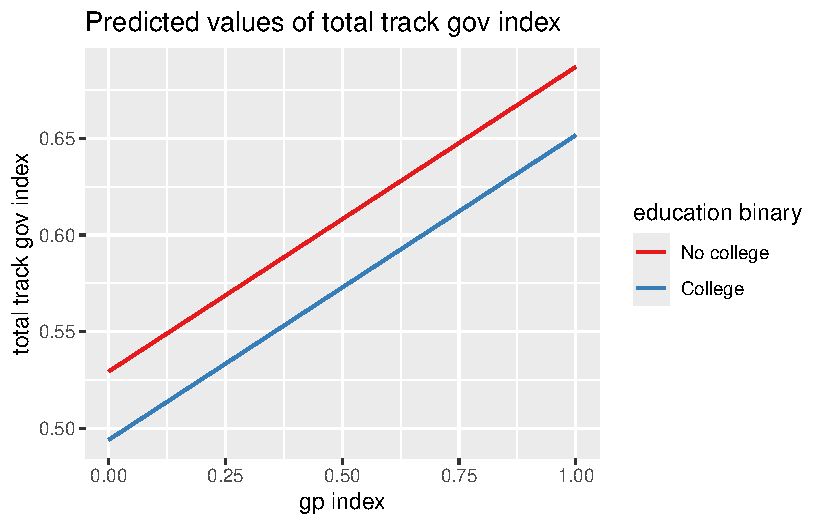
\includegraphics{fig-marginplotperform-1.pdf}

}

\subcaption{\label{fig-marginplotperform-1}GPI x education}

\centering{

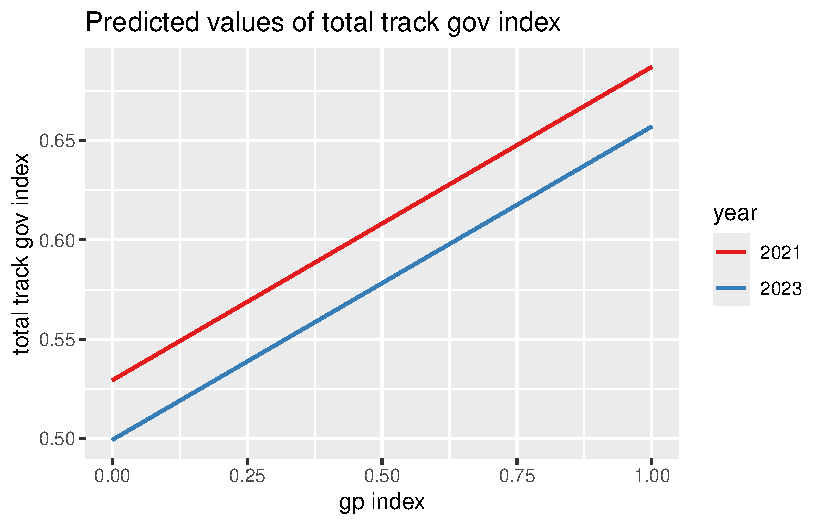
\includegraphics{fig-marginplotperform-2.pdf}

}

\subcaption{\label{fig-marginplotperform-2}GPI x year}

}

\caption{\label{fig-marginplotperform}Marginal effect plots of
interaction terms}

\end{figure}%

As expected, government performance, when controlling for demographic
factors, is a relatively strong predictor of the acceptance of
government surveillance. The model suggests that a positive view of
government performance is associated with an increased acceptance of
government monitoring. However, this relationship could be more complex
than a simple multiple variable regression specification. To further
examine how these factors influence one another, the next section
introduces a mediation model aimed at understanding how the relationship
may have evolved owing to the events of 2022.

\subsection{Changing attitudes since the
pandemic}\label{changing-attitudes-since-the-pandemic}

The following directed acyclic graph (DAG) indicates the hypothesized
causal process that generates the observed outcome variable, tracking
acceptance. In Figure~\ref{fig-dag}, \texttt{TA} represents tracking
acceptance, \texttt{GP} represents government performance approval,
\texttt{DEMO} represents demographic characteristics, and \texttt{COVID}
represents respondents' Covid-19 experience.

To operationalize this model, the first step is to create a latent
demographics construct with the demographic variables previously used in
regressions in the earlier sections loading onto this construct.
\texttt{COVID} is operationalized by the \texttt{year} variable.
Admittedly, this is not a precise operationalization of the Covid
experience - the \texttt{year} variable actually measures all changes
between survey waves not accounted for by other variables. With respect
to government tracking acceptance attitudes, however, this assumption
can be justified by the fact that the Covid-19 experience was both a
daily and often traumatic one for the Chinese public; it was a time
period that involved constant and invasive technological monitoring. If
the model does indicate that the \texttt{year} variable predicts
significant change in the response variable over the two year difference
between survey waves, it would be hard to imagine any other plausible
cause as no other large shifts in technological control existed in the
roughly two years between survey waves. Nevertheless, it is important to
keep in mind that it is only a proxy measurement. These variables
(\texttt{year} for \texttt{COVID}, \texttt{GP}, \texttt{TA}, and
\texttt{DEMO}) are entered into a structural equation model with paths
constrained to that described by the DAG in Figure~\ref{fig-dag} and
then the parameters are estimated using the \texttt{lavaan} library in
\texttt{R}.

\begin{figure}

\centering{

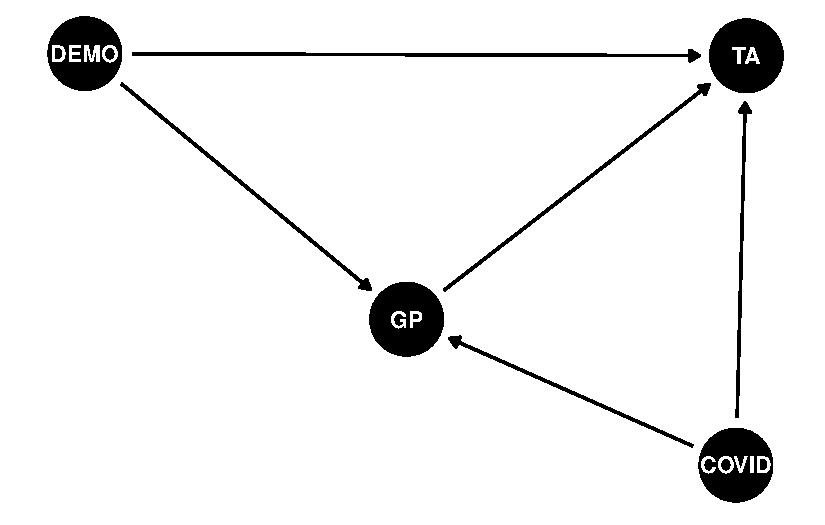
\includegraphics{fig-dag-1.pdf}

}

\caption{\label{fig-dag}Causal process}

\end{figure}%

\begin{table}

\caption{\label{tbl-mediationmodel}Mediation model results}

\centering{

\centering
\begin{tabular}[t]{lc}
\toprule
  & (1)\\
\midrule
DEMO to GP & \num{-0.008}\\
 & \vphantom{1} (\num{0.005})\\
GP to TA & \num{0.430}***\\
 & (\num{0.015})\\
DEMO to TA & \num{-0.010}*\\
 & (\num{0.005})\\
COVID to TA & \num{0.053}***\\
 & (\num{0.006})\\
COVID to GP & \num{-0.037}***\\
 & (\num{0.007})\\
DEMO to GP to TA & \num{-0.003}\\
 & (\num{0.002})\\
COVID to GP to TA & \num{-0.002}***\\
 & (\num{0.000})\\
\midrule
Num.Obs. & \num{3507}\\
AIC & \num{52129.6}\\
BIC & \num{52246.7}\\
\bottomrule
\multicolumn{2}{l}{\rule{0pt}{1em}+ p $<$ 0.1, * p $<$ 0.05, ** p $<$ 0.01, *** p $<$ 0.001}\\
\multicolumn{2}{l}{\rule{0pt}{1em}Demographic factor variable loadings omitted}\\
\end{tabular}

}

\end{table}%

The results from the analysis in Table~\ref{tbl-mediationmodel} confirm
some previous findings and also reveal some interesting new features of
the data. As before, government performance plays a crucial role in
determining tracking acceptance. Similarly, demographic factors do help
predict tracking acceptance, but only slightly. Demographics do not aid
in predicting views on government performance, so it is unsurprising
that demographics do not have an indirect effect on tracking acceptance
through government performance either. However, the Covid-19 experience,
as operationalized by the year variable, 1) positively increases
tracking acceptance (direct path), 2) negatively reduces government
performance evaluations (direct path), and 3) negatively decreases
tracking acceptance through government performance evaluations (indirect
path). The size of the coefficients indicates that the sum of the
effects is still positive on tracking acceptance. These results suggest
that the Covid-19 experience in China did have the effect identified by
\citep{you2024}, which resulted in the hypothesized decrease in
acceptance of government tracking. However, this decrease in support was
offset by the direct effect of Covid-19 on the acceptance of tracking. A
plausible interpretation of this is that respondents agree with
\citep{kostka2024}'s finding: the tracking during Covid-19 lockdowns was
deemed necessary, but due to the government's incompetence in responding
to the spread of the virus, they were less likely to positively agree
than they might otherwise have been.

\subsection{Comparing attitudes to private
monitoring}\label{comparing-attitudes-to-private-monitoring}

Finally, it is interesting to compare the determinants of government
tracking attitudes with those that determine attitudes toward private
tracking of personal information. To compare these two sets of
attitudes, Table~\ref{tbl-privatepublic} includes models that use the
previous acceptance of government tracking index (\texttt{Public\ TA})
as the variable alongside a similarly constructed index variable that
measures acceptance of private monitoring (\texttt{Private\ TA}).

\begin{table}[H]

\caption{\label{tbl-privatepublic}Comparison of public vs.~private
tracking acceptance}

\centering{

\centering
\begin{tabular}[t]{lcccccc}
\toprule
\multicolumn{1}{c}{ } & \multicolumn{3}{c}{Public TA} & \multicolumn{3}{c}{Private TA} \\
\cmidrule(l{3pt}r{3pt}){2-4} \cmidrule(l{3pt}r{3pt}){5-7}
  & (1a) & (1b) & (1c) & (2a) & (2b) & (2c)\\
\midrule
(Intercept) & \num{0.488}*** & \num{0.576}*** & \num{0.214}*** & \num{0.270}*** & \num{0.432}*** & \num{0.344}***\\
 & (\num{0.021}) & (\num{0.022}) & (\num{0.021}) & (\num{0.025}) & (\num{0.026}) & (\num{0.027})\\
Age & \num{0.002}*** & \num{0.001}*** & \num{0.001}** & \num{0.000} & \num{-0.001}** & \num{-0.001}**\\
 & (\num{0.000}) & (\num{0.000}) & (\num{0.000}) & (\num{0.000}) & (\num{0.000}) & (\num{0.000})\\
College education & \num{0.006} & \num{0.014}+ & \num{0.012}+ & \num{-0.027}** & \num{-0.010} & \num{-0.010}\\
 & (\num{0.008}) & (\num{0.008}) & (\num{0.007}) & (\num{0.009}) & (\num{0.009}) & \vphantom{1} (\num{0.009})\\
Middle income & \num{-0.003} & \num{0.001} & \num{-0.003} & \num{-0.059}*** & \num{-0.049}*** & \num{-0.049}***\\
 & (\num{0.008}) & (\num{0.008}) & (\num{0.007}) & (\num{0.009}) & (\num{0.009}) & (\num{0.009})\\
High income & \num{-0.024} & \num{-0.014} & \num{-0.013} & \num{-0.027} & \num{-0.004} & \num{-0.002}\\
 & (\num{0.017}) & (\num{0.017}) & (\num{0.015}) & (\num{0.019}) & (\num{0.020}) & (\num{0.020})\\
Male & \num{-0.009} & \num{-0.004} & \num{-0.005} & \num{-0.006} & \num{0.006} & \num{0.007}\\
 & (\num{0.007}) & (\num{0.007}) & (\num{0.006}) & (\num{0.008}) & (\num{0.008}) & \vphantom{1} (\num{0.008})\\
Not a party member & \num{-0.030}** & \num{-0.032}** & \num{-0.028}** & \num{-0.010} & \num{-0.016} & \num{-0.017}\\
 & (\num{0.010}) & (\num{0.010}) & (\num{0.009}) & (\num{0.012}) & (\num{0.012}) & (\num{0.012})\\
Location: small city & \num{-0.003} & \num{0.002} & \num{-0.006} & \num{-0.043}** & \num{-0.032}* & \num{-0.033}*\\
 & (\num{0.011}) & (\num{0.011}) & (\num{0.010}) & (\num{0.013}) & (\num{0.013}) & (\num{0.013})\\
Location: mid city & \num{0.000} & \num{0.008} & \num{-0.001} & \num{-0.056}*** & \num{-0.038}** & \num{-0.039}**\\
 & (\num{0.012}) & (\num{0.012}) & (\num{0.011}) & (\num{0.014}) & (\num{0.014}) & (\num{0.014})\\
Location: big city & \num{0.001} & \num{0.013} & \num{0.011} & \num{-0.051}*** & \num{-0.024}+ & \num{-0.024}+\\
 & (\num{0.012}) & (\num{0.012}) & (\num{0.010}) & (\num{0.014}) & (\num{0.014}) & (\num{0.014})\\
Year 2023 & \num{0.039}*** & \num{0.036}*** & \num{0.052}*** & \num{0.006} & \num{0.001} & \num{0.005}\\
 & (\num{0.007}) & (\num{0.007}) & (\num{0.006}) & (\num{0.008}) & (\num{0.008}) & (\num{0.008})\\
TSI & \num{0.118}*** &  &  & \num{0.252}*** &  & \\
 & (\num{0.017}) &  &  & (\num{0.021}) &  & \\
KI &  & \num{-0.058}** &  &  & \num{-0.069}** & \\
 &  & (\num{0.022}) &  &  & (\num{0.027}) & \\
GPI &  &  & \num{0.431}*** &  &  & \num{0.071}***\\
 &  &  & (\num{0.015}) &  &  & (\num{0.020})\\
\midrule
Num.Obs. & \num{3507} & \num{3507} & \num{3507} & \num{3507} & \num{3507} & \num{3507}\\
R2 & \num{0.029} & \num{0.018} & \num{0.207} & \num{0.057} & \num{0.018} & \num{0.020}\\
F & \num{9.539} & \num{5.928} & \num{82.827} & \num{19.081} & \num{5.865} & \num{6.450}\\
\bottomrule
\multicolumn{7}{l}{\rule{0pt}{1em}+ p $<$ 0.1, * p $<$ 0.05, ** p $<$ 0.01, *** p $<$ 0.001}\\
\multicolumn{7}{l}{\rule{0pt}{1em}Reference values: no college education, low income, female, party member, countryside}\\
\multicolumn{7}{l}{\rule{0pt}{1em}Standard deviation of Public TA is:  0.2}\\
\multicolumn{7}{l}{\rule{0pt}{1em}Standard deviation of Private TA is:  0.24}\\
\end{tabular}

}

\end{table}%

The results here suggest that the determinants of attitudes towards
private company tracking are somewhat different than those that
determine attitudes towards public tracking. The \texttt{year} variable
is not significant for the private tracking models, while the tech savvy
coefficient has roughly doubled. Unsurprisingly, government performance
is also not related to private tracking acceptance. Finally, the
intercept is generally lower for private tracking acceptance, indicating
that respondents are less willing to accept private tracking, all things
being equal.

These results lend support to the hypothesis that acceptance of public
tracking has different determinants than those for private tracking and
also supports previous research that finds a significant difference
between acceptance of these two types of monitoring. The \texttt{year}
variable being insignificant for the private tracking indicates that the
pandemic-era tracking was not perceived as being fundamentally related
to commercial monitoring.

\section{Conclusion}\label{sec-conclusion}

China's experience with Covid-19 has significantly altered attitudes
towards government tracking---despite a decrease in trust in the state,
overall support for tracking increased. Demographic and informational
variables do not provide strong predictive power for attitudes towards
government tracking. Additionally, the factors that predict acceptance
of government tracking do not show a meaningful correlation with
acceptance of private tracking.

These results carry significant implications for the current body of
literature. Contrary to the literature on demographic characteristics
and privacy, this study found that demographic variables have very
little predictive power, whether they are personal variables or measures
of technological knowledge. This indicates that generalized privacy
attitudes may have determinants that differ from those influencing
attitudes toward government monitoring in China. Such a conclusion
aligns with research by Nam and Steinfeld on American attitudes towards
privacy \citep{nam2019, steinfeld2017}. Furthermore, while the finding
that government trust is a strong predictor of attitudes is consistent
with much of the existing literature, the idea that public events can
significantly shift attitudes is a novel contribution. \citep{davis2004}
suggested that 9/11 may have established a critical context that
influenced whether respondents deemed surveillance necessary and
acceptable, which is compatible with the findings of this study. Lastly,
while the determinants of acceptance for private tracking in China
require more investigation than what is presented here, they appear to
differ considerably from those of government tracking, suggesting
distinct underlying mechanisms at play.

One limitation of this research is that it inquires solely about
generalized acceptance of tracking. \citep{kostka2021} is among the few
studies to concentrate on specific technological applications, such as
facial recognition technology. Further research into the specific
technological methods and aspects of privacy that generate variations in
acceptance would be beneficial. Moreover, this study exclusively
addressed a crisis context where trust in government declined but the
public nonetheless acknowledged the general societal necessity for the
technology. Analyses of other scenarios, involving changes in government
trust levels paired with variations in public acceptance of
technological monitoring, could reinforce the conclusions of this work.

The study suggests that context and the independent acceptance of the
rationale for tracking both significantly impact attitudes towards
online privacy. This is a crucial insight for governments to consider,
as AI and big data continue to expand the interactions between citizens
and state authorities.

\newpage{}

\section{References}\label{references}

\renewcommand{\bibsection}{}
\begin{thebibliography}{10}
\expandafter\ifx\csname url\endcsname\relax
  \def\url#1{\texttt{#1}}\fi
\expandafter\ifx\csname urlprefix\endcsname\relax\def\urlprefix{URL }\fi
\expandafter\ifx\csname href\endcsname\relax
  \def\href#1#2{#2} \def\path#1{#1}\fi

\bibitem{mcmorrow2022}
R.~McMorrow, C.~Leng, \href{https://www.ft.com/content/dee6bcc6-3fc5-4edc-814d-46dc73e67c7e}{{\textquoteleft}digital handcuffs{\textquoteright}: China{\textquoteright}s covid health apps govern life but are ripe for abuse}, Financial Times (06 2022).
\newline\urlprefix\url{https://www.ft.com/content/dee6bcc6-3fc5-4edc-814d-46dc73e67c7e}

\bibitem{gómez-barroso2018}
J.~{Gómez-Barroso}, \href{https://www.sciencedirect.com/science/article/pii/S0736585318302107}{Experiments on personal information disclosure: Past and future avenues}, Telematics and Informatics 35~(5) (2018) 1473--1490.
\newblock \href {https://doi.org/10.1016/j.tele.2018.03.017} {\path{doi:10.1016/j.tele.2018.03.017}}.
\newline\urlprefix\url{https://www.sciencedirect.com/science/article/pii/S0736585318302107}

\bibitem{reddick2015}
C.~G. Reddick, A.~T. Chatfield, P.~A. Jaramillo, \href{https://www.sciencedirect.com/science/article/pii/S0740624X15000246}{Public opinion on national security agency surveillance programs: A multi-method approach}, Government Information Quarterly 32~(2) (2015) 129--141.
\newblock \href {https://doi.org/10.1016/j.giq.2015.01.003} {\path{doi:10.1016/j.giq.2015.01.003}}.
\newline\urlprefix\url{https://www.sciencedirect.com/science/article/pii/S0740624X15000246}

\bibitem{sheehan2002}
K.~B. Sheehan, \href{https://doi.org/10.1080/01972240252818207}{Toward a typology of internet users and online privacy concerns}, The Information Society 18~(1) (2002) 21--32, publisher: Routledge {\_}eprint: https://doi.org/10.1080/01972240252818207.
\newblock \href {https://doi.org/10.1080/01972240252818207} {\path{doi:10.1080/01972240252818207}}.
\newline\urlprefix\url{https://doi.org/10.1080/01972240252818207}

\bibitem{anwar2017}
M.~Anwar, W.~He, I.~Ash, X.~Yuan, L.~Li, L.~Xu, \href{https://www.sciencedirect.com/science/article/pii/S0747563216308688}{Gender difference and employees' cybersecurity behaviors}, Computers in Human Behavior 69 (2017) 437--443.
\newblock \href {https://doi.org/10.1016/j.chb.2016.12.040} {\path{doi:10.1016/j.chb.2016.12.040}}.
\newline\urlprefix\url{https://www.sciencedirect.com/science/article/pii/S0747563216308688}

\bibitem{büchi2021}
M.~{Büchi}, N.~Festic, N.~Just, M.~Latzer, Digital inequalities in online privacy protection: effects of age, education and gender, Edward Elgar Publishing, 2021, p. 296{\textendash}310.

\bibitem{lee2019}
H.~Lee, S.~F. Wong, J.~Oh, Y.~Chang, \href{https://www.sciencedirect.com/science/article/pii/S0740624X18303265}{Information privacy concerns and demographic characteristics: Data from a korean media panel survey}, Government Information Quarterly 36~(2) (2019) 294--303.
\newblock \href {https://doi.org/10.1016/j.giq.2019.01.002} {\path{doi:10.1016/j.giq.2019.01.002}}.
\newline\urlprefix\url{https://www.sciencedirect.com/science/article/pii/S0740624X18303265}

\bibitem{baskaran2024}
K.~Baskaran, S.~K. Mathew, \href{https://doi.org/10.1080/10447318.2022.2124358}{Understanding coping intentions of fitness tracker users: An empirical investigation using fear appeals}, International Journal of Human{\textendash}Computer Interaction 40~(3) (2024) 795--807, publisher: Taylor \& Francis {\_}eprint: https://doi.org/10.1080/10447318.2022.2124358.
\newblock \href {https://doi.org/10.1080/10447318.2022.2124358} {\path{doi:10.1080/10447318.2022.2124358}}.
\newline\urlprefix\url{https://doi.org/10.1080/10447318.2022.2124358}

\bibitem{dupree2016}
J.~L. Dupree, R.~Devries, D.~M. Berry, E.~Lank, \href{https://dl.acm.org/doi/10.1145/2858036.2858214}{Privacy personas: Clustering users via attitudes and behaviors toward security practices}, CHI '16, Association for Computing Machinery, New York, NY, USA, 2016, p. 5228{\textendash}5239.
\newblock \href {https://doi.org/10.1145/2858036.2858214} {\path{doi:10.1145/2858036.2858214}}.
\newline\urlprefix\url{https://dl.acm.org/doi/10.1145/2858036.2858214}

\bibitem{kokolakis2017}
S.~Kokolakis, \href{https://www.sciencedirect.com/science/article/pii/S0167404815001017}{Privacy attitudes and privacy behaviour: A review of current research on the privacy paradox phenomenon}, Computers \& Security 64 (2017) 122--134.
\newblock \href {https://doi.org/10.1016/j.cose.2015.07.002} {\path{doi:10.1016/j.cose.2015.07.002}}.
\newline\urlprefix\url{https://www.sciencedirect.com/science/article/pii/S0167404815001017}

\bibitem{blank}
G.~Blank, G.~Bolsover, E.~Dubois, A new privacy paradox: Young people and privacy on social network sites\href {https://doi.org/10.2139/ssrn.2479938} {\path{doi:10.2139/ssrn.2479938}}.

\bibitem{davis2004}
D.~W. Davis, B.~D. Silver, \href{https://onlinelibrary.wiley.com/doi/abs/10.1111/j.0092-5853.2004.00054.x}{Civil liberties vs. security: Public opinion in the context of the terrorist attacks on america}, American Journal of Political Science 48~(1) (2004) 28--46, {\_}eprint: https://onlinelibrary.wiley.com/doi/pdf/10.1111/j.0092-5853.2004.00054.x.
\newblock \href {https://doi.org/10.1111/j.0092-5853.2004.00054.x} {\path{doi:10.1111/j.0092-5853.2004.00054.x}}.
\newline\urlprefix\url{https://onlinelibrary.wiley.com/doi/abs/10.1111/j.0092-5853.2004.00054.x}

\bibitem{pavone2012}
V.~Pavone, S.~D. Esposti, \href{https://doi.org/10.1177/0963662510376886}{Public assessment of new surveillance-oriented security technologies: Beyond the trade-off between privacy and security}, Public Understanding of Science 21~(5) (2012) 556--572, publisher: SAGE Publications Ltd.
\newblock \href {https://doi.org/10.1177/0963662510376886} {\path{doi:10.1177/0963662510376886}}.
\newline\urlprefix\url{https://doi.org/10.1177/0963662510376886}

\bibitem{trüdinger2017}
E.-M. {Trüdinger}, L.~C. Steckermeier, \href{https://www.sciencedirect.com/science/article/pii/S0740624X16303173}{Trusting and controlling? political trust, information and acceptance of surveillance policies: The case of germany}, Government Information Quarterly 34~(3) (2017) 421--433.
\newblock \href {https://doi.org/10.1016/j.giq.2017.07.003} {\path{doi:10.1016/j.giq.2017.07.003}}.
\newline\urlprefix\url{https://www.sciencedirect.com/science/article/pii/S0740624X16303173}

\bibitem{abramova2022}
O.~Abramova, A.~Wagner, C.~M. Olt, P.~Buxmann, \href{https://www.sciencedirect.com/science/article/pii/S0268401222000044}{One for all, all for one: Social considerations in user acceptance of contact tracing apps using longitudinal evidence from germany and switzerland}, International Journal of Information Management 64 (2022) 102473.
\newblock \href {https://doi.org/10.1016/j.ijinfomgt.2022.102473} {\path{doi:10.1016/j.ijinfomgt.2022.102473}}.
\newline\urlprefix\url{https://www.sciencedirect.com/science/article/pii/S0268401222000044}

\bibitem{garrett2021}
P.~M. Garrett, J.~P. White, S.~Lewandowsky, Y.~Kashima, A.~Perfors, D.~R. Little, N.~Geard, L.~Mitchell, M.~Tomko, S.~Dennis, \href{https://journals.plos.org/plosone/article?id=10.1371/journal.pone.0244827}{The acceptability and uptake of smartphone tracking for covid-19 in australia}, PLOS ONE 16~(1) (2021) e0244827, publisher: Public Library of Science.
\newblock \href {https://doi.org/10.1371/journal.pone.0244827} {\path{doi:10.1371/journal.pone.0244827}}.
\newline\urlprefix\url{https://journals.plos.org/plosone/article?id=10.1371/journal.pone.0244827}

\bibitem{ioannou2021}
A.~Ioannou, I.~Tussyadiah, \href{https://www.sciencedirect.com/science/article/pii/S0160791X21002499}{Privacy and surveillance attitudes during health crises: Acceptance of surveillance and privacy protection behaviours}, Technology in Society 67 (2021) 101774.
\newblock \href {https://doi.org/10.1016/j.techsoc.2021.101774} {\path{doi:10.1016/j.techsoc.2021.101774}}.
\newline\urlprefix\url{https://www.sciencedirect.com/science/article/pii/S0160791X21002499}

\bibitem{ong}
E.-I. Ong, W.~L. Loo, Gauging the acceptance of contact tracing technology: An empirical study of singapore residents' concerns and trust in information sharing\href {https://doi.org/10.2139/ssrn.3817972} {\path{doi:10.2139/ssrn.3817972}}.

\bibitem{wnuk2020}
A.~Wnuk, T.~Oleksy, D.~Maison, \href{https://journals.plos.org/plosone/article?id=10.1371/journal.pone.0238973}{The acceptance of covid-19 tracking technologies: The role of perceived threat, lack of control, and ideological beliefs}, PLOS ONE 15~(9) (2020) e0238973, publisher: Public Library of Science.
\newblock \href {https://doi.org/10.1371/journal.pone.0238973} {\path{doi:10.1371/journal.pone.0238973}}.
\newline\urlprefix\url{https://journals.plos.org/plosone/article?id=10.1371/journal.pone.0238973}

\bibitem{habich-sobiegalla2023}
S.~Habich-Sobiegalla, G.~Kostka, \href{https://doi.org/10.1080/1369118X.2022.2113421}{Sharing is caring: willingness to share personal data through contact tracing apps in china, germany, and the us}, Information, Communication \& Society 26~(14) (2023) 2797--2824, publisher: Routledge {\_}eprint: https://doi.org/10.1080/1369118X.2022.2113421.
\newblock \href {https://doi.org/10.1080/1369118X.2022.2113421} {\path{doi:10.1080/1369118X.2022.2113421}}.
\newline\urlprefix\url{https://doi.org/10.1080/1369118X.2022.2113421}

\bibitem{kostka2021}
G.~Kostka, L.~Steinacker, M.~Meckel, \href{https://doi.org/10.1177/09636625211001555}{Between security and convenience: Facial recognition technology in the eyes of citizens in china, germany, the united kingdom, and the united states}, Public Understanding of Science 30~(6) (2021) 671--690, publisher: SAGE Publications Ltd.
\newblock \href {https://doi.org/10.1177/09636625211001555} {\path{doi:10.1177/09636625211001555}}.
\newline\urlprefix\url{https://doi.org/10.1177/09636625211001555}

\bibitem{kostka2024}
G.~Kostka, S.~Habich-Sobiegalla, \href{https://doi.org/10.1177/14614448221083285}{In times of crisis: Public perceptions toward covid-19 contact tracing apps in china, germany, and the united states}, New Media \& Society 26~(4) (2024) 2256--2294, publisher: SAGE Publications.
\newblock \href {https://doi.org/10.1177/14614448221083285} {\path{doi:10.1177/14614448221083285}}.
\newline\urlprefix\url{https://doi.org/10.1177/14614448221083285}

\bibitem{kostka2023}
G.~Kostka, \href{https://www.cambridge.org/core/journals/data-and-policy/article/digital-doubters-in-different-political-and-cultural-contexts-comparing-citizen-attitudes-across-three-major-digital-technologies/EF171C5121F6E1175554D32D23CD297E}{Digital doubters in different political and cultural contexts: Comparing citizen attitudes across three major digital technologies}, Data \& Policy 5 (2023) e27, publisher: Cambridge University Press.
\newblock \href {https://doi.org/10.1017/dap.2023.25} {\path{doi:10.1017/dap.2023.25}}.
\newline\urlprefix\url{https://www.cambridge.org/core/journals/data-and-policy/article/digital-doubters-in-different-political-and-cultural-contexts-comparing-citizen-attitudes-across-three-major-digital-technologies/EF171C5121F6E1175554D32D23CD297E}

\bibitem{liu2022}
C.~Liu, \href{https://doi.org/10.1177/02685809221084446}{Who supports expanding surveillance? exploring public opinion of chinese social credit systems}, International Sociology 37~(3) (2022) 391--412, publisher: SAGE Publications Ltd.
\newblock \href {https://doi.org/10.1177/02685809221084446} {\path{doi:10.1177/02685809221084446}}.
\newline\urlprefix\url{https://doi.org/10.1177/02685809221084446}

\bibitem{steinfeld2017}
N.~Steinfeld, \href{https://www.sciencedirect.com/science/article/pii/S0736585317303349}{Track me, track me not: Support and consent to state and private sector surveillance}, Telematics and Informatics 34~(8) (2017) 1663--1672.
\newblock \href {https://doi.org/10.1016/j.tele.2017.07.012} {\path{doi:10.1016/j.tele.2017.07.012}}.
\newline\urlprefix\url{https://www.sciencedirect.com/science/article/pii/S0736585317303349}

\bibitem{nam2019}
T.~Nam, \href{https://www.sciencedirect.com/science/article/pii/S0362331918301423}{What determines the acceptance of government surveillance? examining the influence of information privacy correlates}, The Social Science Journal 56~(4) (2019) 530--544.
\newblock \href {https://doi.org/10.1016/j.soscij.2018.10.001} {\path{doi:10.1016/j.soscij.2018.10.001}}.
\newline\urlprefix\url{https://www.sciencedirect.com/science/article/pii/S0362331918301423}

\bibitem{steinhardt2022}
H.~C. Steinhardt, L.~Holzschuh, A.~W. MacDonald, \href{https://firstmonday.org/ojs/index.php/fm/article/view/12679}{Dreading big brother or dreading big profit? privacy concerns toward the state and companies in china}, First Monday (12 2022).
\newblock \href {https://doi.org/10.5210/fm.v27i12.12679} {\path{doi:10.5210/fm.v27i12.12679}}.
\newline\urlprefix\url{https://firstmonday.org/ojs/index.php/fm/article/view/12679}

\bibitem{you2024}
Y.~You, D.~Ma, C.~Chen, \href{https://doi.org/10.1007/s11366-023-09874-y}{Public trust during a public health crisis: Evaluating the immediate effects of the pandemic on institutional trust}, Journal of Chinese Political Science 29~(1) (2024) 1--29.
\newblock \href {https://doi.org/10.1007/s11366-023-09874-y} {\path{doi:10.1007/s11366-023-09874-y}}.
\newline\urlprefix\url{https://doi.org/10.1007/s11366-023-09874-y}

\bibitem{han2018}
R.~Han, \href{https://www.degruyter.com/document/doi/10.7312/han-18474/html}{Contesting Cyberspace in China: Online Expression and Authoritarian Resilience}, Columbia University Press, 2018, dOI: 10.7312/han-18474.
\newblock \href {https://doi.org/10.7312/han-18474} {\path{doi:10.7312/han-18474}}.
\newline\urlprefix\url{https://www.degruyter.com/document/doi/10.7312/han-18474/html}

\bibitem{gainous2023}
J.~Gainous, R.~Han, A.~W. MacDonald, K.~M. Wagner, \href{https://academic.oup.com/book/55291}{Directed Digital Dissidence in Autocracies: How China Wins Online}, Oxford University Press, 2023, dOI: 10.1093/oso/9780197680384.001.0001.
\newblock \href {https://doi.org/10.1093/oso/9780197680384.001.0001} {\path{doi:10.1093/oso/9780197680384.001.0001}}.
\newline\urlprefix\url{https://academic.oup.com/book/55291}

\bibitem{chen2017}
D.~Chen, \href{https://doi.org/10.1177/1065912917691360}{Local distrust and regime support: Sources and effects of political trust in china}, Political Research Quarterly 70~(2) (2017) 314--326, publisher: SAGE Publications Inc.
\newblock \href {https://doi.org/10.1177/1065912917691360} {\path{doi:10.1177/1065912917691360}}.
\newline\urlprefix\url{https://doi.org/10.1177/1065912917691360}

\bibitem{qiu2012}
H.~Qiu, J.~Huang, C.~Pray, S.~Rozelle, \href{https://doi.org/10.1080/14765284.2012.638471}{Consumers{\textquoteright} trust in government and their attitudes towards genetically modified food: empirical evidence from china}, Journal of Chinese Economic and Business Studies 10~(1) (2012) 67--87, publisher: Routledge {\_}eprint: https://doi.org/10.1080/14765284.2012.638471.
\newblock \href {https://doi.org/10.1080/14765284.2012.638471} {\path{doi:10.1080/14765284.2012.638471}}.
\newline\urlprefix\url{https://doi.org/10.1080/14765284.2012.638471}

\bibitem{zhou2018}
Y.~J. Zhou, S.~Jin, \href{https://www.cambridge.org/core/journals/china-quarterly/article/inequality-and-political-trust-in-china-the-social-volcano-thesis-reexamined/27E249A41FF2A5A70EBB37F15AB6709C}{Inequality and political trust in china: The social volcano thesis re-examined}, The China Quarterly 236 (2018) 1033--1062.
\newblock \href {https://doi.org/10.1017/S0305741018001297} {\path{doi:10.1017/S0305741018001297}}.
\newline\urlprefix\url{https://www.cambridge.org/core/journals/china-quarterly/article/inequality-and-political-trust-in-china-the-social-volcano-thesis-reexamined/27E249A41FF2A5A70EBB37F15AB6709C}

\bibitem{wuhanlo2021}
\href{https://www.bbc.com/news/world-asia-china-55628488}{Wuhan lockdown: A year of china's fight against the covid pandemic}, BBC News (01 2021).
\newline\urlprefix\url{https://www.bbc.com/news/world-asia-china-55628488}

\bibitem{mao2022}
F.~Mao, \href{https://www.bbc.com/news/world-asia-china-63855508}{China abandons key parts of zero-covid strategy after protests}, BBC News (12 2022).
\newline\urlprefix\url{https://www.bbc.com/news/world-asia-china-63855508}

\bibitem{zhong2014}
Y.~Zhong, \href{https://www.tandfonline.com/doi/abs/10.2753/PPC1075-8216610303}{Do chinese people trust their local government, and why?}, Problems of Post-CommunismPublisher: Routledge (05 2014).
\newblock \href {https://doi.org/10.2753/PPC1075-8216610303} {\path{doi:10.2753/PPC1075-8216610303}}.
\newline\urlprefix\url{https://www.tandfonline.com/doi/abs/10.2753/PPC1075-8216610303}

\bibitem{carter2024}
E.~B. Carter, B.~L. Carter, S.~Schick, \href{https://www.cambridge.org/core/journals/china-quarterly/article/do-chinese-citizens-conceal-opposition-to-the-ccp-in-surveys-evidence-from-two-experiments/12A2440F948D016E8D845C492F7D0CFE}{Do chinese citizens conceal opposition to the ccp in surveys? evidence from two experiments}, The China Quarterly (2024) 1--10\href {https://doi.org/10.1017/S0305741023001819} {\path{doi:10.1017/S0305741023001819}}.
\newline\urlprefix\url{https://www.cambridge.org/core/journals/china-quarterly/article/do-chinese-citizens-conceal-opposition-to-the-ccp-in-surveys-evidence-from-two-experiments/12A2440F948D016E8D845C492F7D0CFE}

\bibitem{jiang2016}
J.~Jiang, D.~L. Yang, \href{https://doi.org/10.1177/0010414015626450}{Lying or believing? measuring preference falsification from a political purge in china}, Comparative Political Studies 49~(5) (2016) 600--634, publisher: SAGE Publications Inc.
\newblock \href {https://doi.org/10.1177/0010414015626450} {\path{doi:10.1177/0010414015626450}}.
\newline\urlprefix\url{https://doi.org/10.1177/0010414015626450}

\bibitem{ratigan2020}
K.~Ratigan, L.~Rabin, \href{https://www.cambridge.org/core/journals/china-quarterly/article/reevaluating-political-trust-the-impact-of-survey-nonresponse-in-rural-china/05403CA9F41979BD624055E03D9F6FA9}{Re-evaluating political trust: The impact of survey nonresponse in rural china}, The China Quarterly 243 (2020) 823--838.
\newblock \href {https://doi.org/10.1017/S0305741019001231} {\path{doi:10.1017/S0305741019001231}}.
\newline\urlprefix\url{https://www.cambridge.org/core/journals/china-quarterly/article/reevaluating-political-trust-the-impact-of-survey-nonresponse-in-rural-china/05403CA9F41979BD624055E03D9F6FA9}

\bibitem{redlawsk2010}
D.~P. Redlawsk, C.~J. Tolbert, W.~Franko, \href{https://doi.org/10.1177/1065912910373554}{Voters, emotions, and race in 2008: Obama as the first black president}, Political Research Quarterly 63~(4) (2010) 875--889, publisher: SAGE Publications Inc.
\newblock \href {https://doi.org/10.1177/1065912910373554} {\path{doi:10.1177/1065912910373554}}.
\newline\urlprefix\url{https://doi.org/10.1177/1065912910373554}

\bibitem{moseson2017}
H.~Moseson, E.~Treleaven, C.~Gerdts, N.~Diamond-Smith, \href{https://onlinelibrary.wiley.com/doi/abs/10.1111/sifp.12042}{The list experiment for measuring abortion: What we know and what we need}, Studies in Family Planning 48~(4) (2017) 397--405, {\_}eprint: https://onlinelibrary.wiley.com/doi/pdf/10.1111/sifp.12042.
\newblock \href {https://doi.org/10.1111/sifp.12042} {\path{doi:10.1111/sifp.12042}}.
\newline\urlprefix\url{https://onlinelibrary.wiley.com/doi/abs/10.1111/sifp.12042}

\bibitem{glynn2013}
A.~N. Glynn, \href{https://academic.oup.com/poq/article/77/S1/159/1878470/What-Can-We-Learn-with-Statistical-Truth-Serum}{What can we learn with statistical truth serum?design and analysis of the list experiment}, Public Opinion Quarterly 77~(S1) (2013) 159--172.
\newblock \href {https://doi.org/10.1093/poq/nfs070} {\path{doi:10.1093/poq/nfs070}}.
\newline\urlprefix\url{https://academic.oup.com/poq/article/77/S1/159/1878470/What-Can-We-Learn-with-Statistical-Truth-Serum}

\bibitem{harmel2019}
R.~Harmel, Y.-Y. Yeh, X.~Liu, \href{https://onlinelibrary.wiley.com/doi/abs/10.1111/ssqu.12681}{Age versus socialization in understanding attitudes toward economic reforms in china}, Social Science Quarterly 100~(5) (2019) 1755--1767, {\_}eprint: https://onlinelibrary.wiley.com/doi/pdf/10.1111/ssqu.12681.
\newblock \href {https://doi.org/10.1111/ssqu.12681} {\path{doi:10.1111/ssqu.12681}}.
\newline\urlprefix\url{https://onlinelibrary.wiley.com/doi/abs/10.1111/ssqu.12681}

\bibitem{steinhardt2020}
H.~C. Steinhardt, J.~Delhey, \href{https://doi.org/10.1007/s11205-020-02466-w}{Socio-economic modernization and the {\textquotedblleft}crisis of trust{\textquotedblright} in china: A multi-level analysis of general and particular trust}, Social Indicators Research 152~(3) (2020) 923--949.
\newblock \href {https://doi.org/10.1007/s11205-020-02466-w} {\path{doi:10.1007/s11205-020-02466-w}}.
\newline\urlprefix\url{https://doi.org/10.1007/s11205-020-02466-w}

\end{thebibliography}


\newpage{}

\section{Appendix}\label{sec-appendix}

\subsection{Index variable
definitions}\label{index-variable-definitions}

\begin{table}[H]

\caption{\label{tbl-tsindexvars}Tech savvy index variable construction}

\centering{

\centering
\begin{tabular}[t]{l|l}
\hline
Q1 & How would you rate your general ability to use a computer?\\
\hline
\cellcolor{gray!6}{Q2} & \cellcolor{gray!6}{How would you rate your skill at fixing a computer?}\\
\hline
Q3 & How would you rate your ability to program a computer?\\
\hline
\end{tabular}

}

\end{table}%

\begin{table}[H]

\caption{\label{tbl-pkindexvars}Privacy knowledge index variable
construction}

\centering{

\centering
\begin{tabular}[t]{l|l}
\hline
Q1 & I am very concerned about my privacy online\\
\hline
\cellcolor{gray!6}{Q2} & \cellcolor{gray!6}{I spend a lot of time reading about technology related privacy issues}\\
\hline
Q3 & In the last year, I have had discussions with my friends about online privacy issues\\
\hline
\cellcolor{gray!6}{Q4} & \cellcolor{gray!6}{I feel like I know exactly how much privacy I have online}\\
\hline
Q5 & Have you heard of the social credit system (official terminology)?\\
\hline
\end{tabular}

}

\end{table}%

\begin{table}[H]

\caption{\label{tbl-gpindexvars}Government performance index variable
construction}

\centering{

\centering
\begin{tabular}[t]{l|>{\raggedright\arraybackslash}p{5in}}
\hline
Q1 & Overall, I’m happy with the performance of the central government\\
\hline
\cellcolor{gray!6}{Q2} & \cellcolor{gray!6}{Overall, I’m happy with the performance of my local government}\\
\hline
\end{tabular}

}

\end{table}%




\end{document}
